\chapter{Summary}
Das Projekt BestShift wird wie folgt durchgeführt:
<<<<<<< HEAD
<<<<<<< HEAD
	\begin{itemize}
		\item Tobias Perny: Hardware und Sensorik in Form eines Raspberry Pi's und verschiedenen Sensoren 
		\item Daniel Melichar: Data Mining und Data Management mithilfe von Couchbase in der NoSQL-Variante
		\item Hüseyin Bozkurt: Webapplikation mittels Python(plotly), Java Smartphone/Webapplikation mittels MPAndroidChart, Kapitel Verbrauchsanalyse 
		\item Raphael Simsek:  Webapplikation mittels Python(plotly), Java Smartphone/Webapplikation mittels MPAndroidChart, Kapitel Fahrgastbequemlichkeit
		\item Fitim Faiku:     Webapplikation mittels Python(plotly), Java Smartphone/Webapplikation mittels MPAndroidChart, Kapitel Schaltvorschlag
	\end{itemize}

=======
=======
>>>>>>> 71c215f004964c57cf89ee1fdf8056a02969acb9
\section{Zusammenstellung der Aufgabenverteilung}
 \begin{itemize}
	 \item Tobias Perny: Hardware und Sensorik in Form eines Raspberry Pi's und verschiedenen Sensoren 
	 \item Daniel Melichar: Data Mining und Data Management mithilfe von Couchbase in der NoSQL-Variante
	 \item Hüseyin Bozkurt: Webapplikation mittels Python(plotly), Java Smartphone-/Webapplikation mittels MPAndroidChart, Kapitel Momentane Verbrauchsanalyse mittels verschiedenen Graph-Elementen, welche auf der Webapplikation auch zu Retrospektiven Zwecken verwendet werden können 
	 \item Raphael Simsek: Webapplikation mittels Python(plotly), Java Smartphone-/Webapplikation mittels MPAndroidChart, Kapitel Schaltvorschlag durch die Anzeige der Drehzahl und des optimalen Ganges in einer grafisch ansprechenden art.
	 \item Fitim Faiku: Webapplikation mittels Python(plotly), Java Smartphone-/Webapplikation mittels MPAndroidChart, Kapitel Fahrgastbequemlichkeit fokussiert sich auf die Anzeige der momentanen Querbeschleunigung mittels eines Kamm'schen Kreises
 \end{itemize}
\newline
\section{Workflowdiagramm}
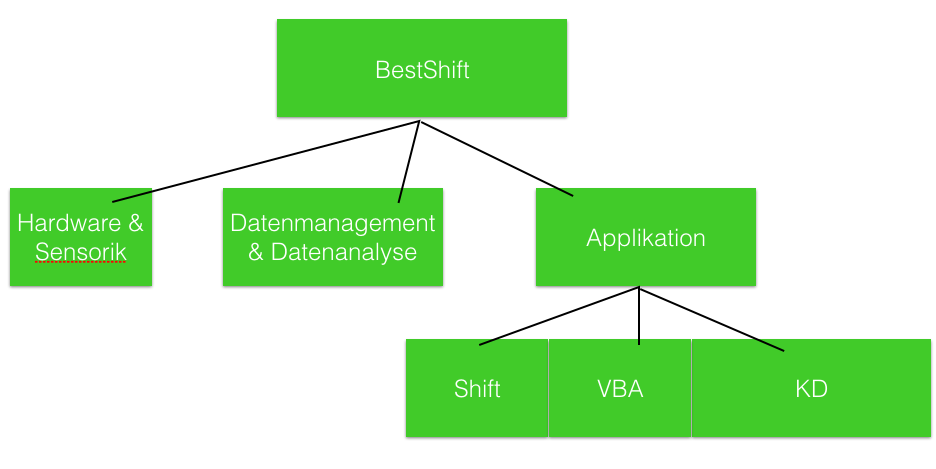
\includegraphics[scale=0.5]{images/Workflowdiagramm.png}

\newline
\section{Workflow des Projektes}
	\subsection{Tobias Perny - Hardware und Sensorik}
	Tobias Perny ist im Projekt wie bereits erwähnt für die Hardware und Sensorik zuständig. Er arbeitet mit einem Raspberry Pi2 Single Board Computer (SBC) auf welchem verschiedene Sensoren direkt montiert sind, welche dann interpretiert werden. Herr Perny verwendet die Programmiersprache Python um die Sensoren anzusprechen und diese mittels der Datenblätter der Sensoren in Informationen umzuwandeln. Diese Werte werden dann von Herrn Melichar endgültig in Einheiten umgesetzt.
	Zusätzlich zu den eigenen Sensoren liest der Raspberry Pi2 außerdem die OBD-II Motordaten aus stellt diese zur Speicherung bereit. 
	Die Auslesung aus dem Motormanagement wird mittels einer Bluetooth Schnittstelle mit einem ELM327-Chip für den OBD-II Port stattfinden.

	\subsection{Daniel Melichar - Datenmanagement und Datenanalyse}
	Die Speicherung der bereitgestellten Daten übernimmt Daniel Melichar, welcher diese weiterverarbeitet indem er die Daten strukturiert in einer Couchbase NoSQL Implementierung ablegt. Zudem stellt Herr Melichar dann Methoden zur Verfügung mit welchen die aktuellsten Daten und die Daten die in Ihrer Auflösung reduziert wurden bereit gestellt werden. Diese Methoden sind für die App Entwicklung von essenzieller Bedeutung, weil dadurch die Verbindung zur Datenbank für die Entwickler erleichtert wird.
	Daniel Melichar ist außerdem für die Datenstrukturierung und das Account Management der geplanten Web-Applikation zuständig. Das Account Management wird erneut mit Hilfe der NoSQL Datenbank Couchbase realisiert. Die Datenstrukturierung wird mittels eines Content Management Systems geschehen, für welches Herr Melichar sich um das Hosting und die Rechte auf dem Server kümmern wird. 

	\subsection{Raphael Simsek - Schaltvorgangsvorschlag}
	Raphael Simsek erstellt das Grundgerüst der App mittels dem Angular JS Framework ionic gemeinsam mit dem App-Team bestehend aus Hüseyin Bozkurt und Fitim Faiku.
	Mit den von Daniel Melichar erstellten Methoden berechnet Raphael Simsek den effizientesten oder drehmomentintensivsten Gang mittels verschiedener Algorithmen. Diese Gang-Berechnung soll allerdings auf aktuelle Erkenntnisse aus dem Motormanagement eingehen, indem beispielsweise die Informationen des Gyroskops für die Erkenntnis ob der Nutzer sich auf einer steilen oder abfallenden Straße befindet um dadurch unnötige Falschangaben der App zu vermeiden. Die Erkennung ob ein Gang wirklich gewechselt wurde soll mittels der stark abfallenden Drehzahl oder der Fahrgeschwindigkeit passieren.
	
	\subsection{Hüseyin Bozkurt - Verbrauchsanalyse}
	 Hüseyin Bozkurt ist für die Verbrauchsdarstellung während der Fahrt und für die retrospektive Verbrauchsanalyse nach der Fahrt zuständig.
	 Diese wird hauptsächlich in Form von Liniendiagrammen geschehen, indem man den Schadstoffausstoß über eine bestimmte Zeit analysiert. In Verbindung mit der Webapplikation, werden diese Informationen mit OpenMap-Daten verbunden und zur schau gestellt.
	 Somit soll eine umweltentlastende Fahrweise nach und nach gefördert werden. Demnach existiert die Option, die analysierte Fahrt auf Facebook mittels OAuth zu teilen, um Mitbenutzern der App einen Vergleich bieten zu können und - falls es Fragen wie zum Beispiel zu einer Strecke gibt, ihnen durch diese Vergleichswerte genügend Information zu bieten und eine offene Diskussionsrunde zu starten.
	
	\subsection{Fitim Faiku - Fahrkomfortanalyse}
	 Fitim Faiku stellt die Fahrgastbequemlichkeit eines KFZ während der Fahrt dar.
	 Dies geschieht in Form eines Kamm'schen Kreises, welches die Längs- und Querbeschleunigung anzeigt. Faiku wird für diese Aufgabe die Programmiersprache Java anwenden.
	 Das Framework MPAndroidChart wird ihm dabei behilflich sein. Bei kurvigen Straßen schlägt der Kreis aus, wodurch der KFZ-Fahrer auf eine Geschwindigkeitsanpassung audiovisuell aufmerksam gemacht wird.
